\begingroup
\begin{center}
\fontsize{15}{15}\sffamily\selectfont
\textbf{Hyperbolic Functions}
\end{center}
\endgroup

\begin{table}[H]
    \centering
    \begin{minipage}[t]{0.45\linewidth}
        \begin{figure}[H]
            \centering
            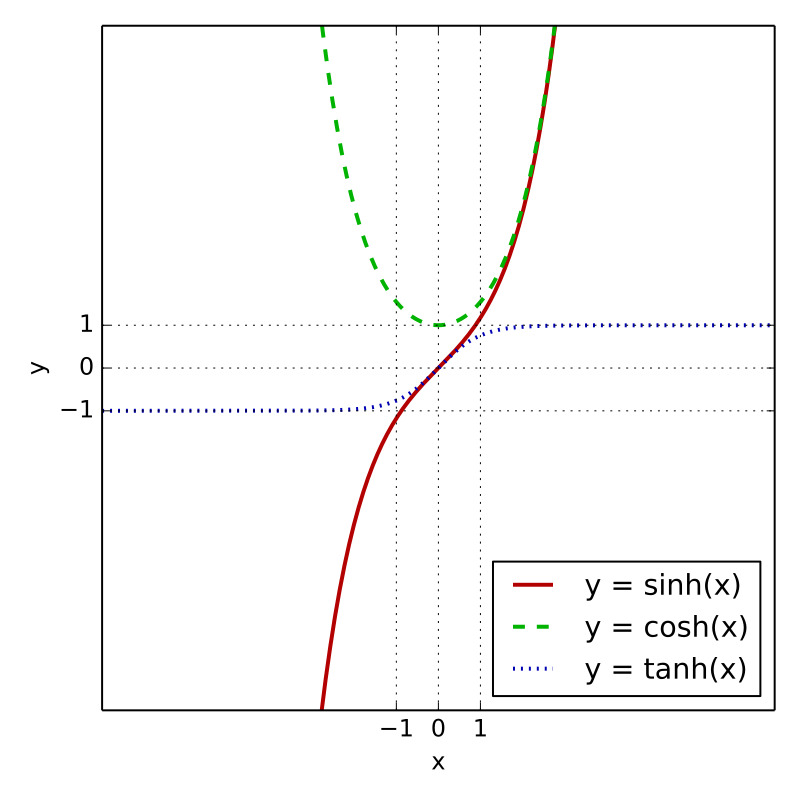
\includegraphics[height=7.5cm]{Pictures/maths/Sinh_cosh_tanh.jpg}
            \caption{$\sinh(x)$, $\cosh(x)$ \& $\tanh(x)$}
        \end{figure}        
    \end{minipage}
    \hfill
    \begin{minipage}[t]{0.45\linewidth}
        \begin{figure}[H]
            \centering
            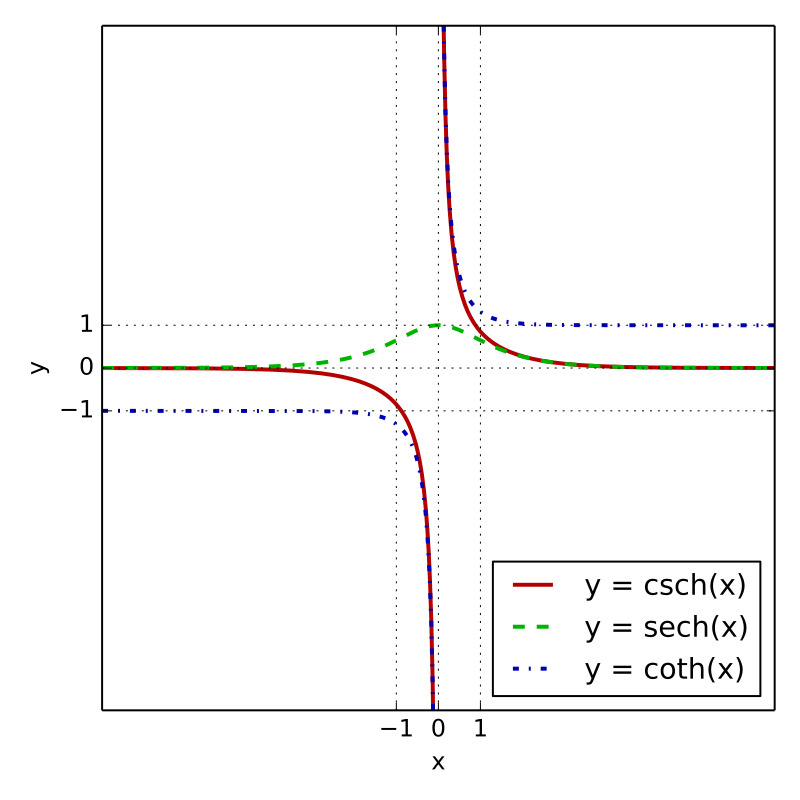
\includegraphics[height=7.5cm]{Pictures/maths/Csch_sech_coth.jpg}
            \caption{$\rcmdXcsch(x)$, $\rcmdXsech(x)$ \& $\coth(x)$}
        \end{figure}
    \end{minipage}
\end{table}

\section{Hyperbolic sine ( $\sinh(x)$ ) }\label{Hyperbolic sine (sinh)}
\[
    (\sinh(x) = {\displaystyle\dfrac{e^{x} - e^{-x}}{2}}={\displaystyle\dfrac{e^{2x} - 1}{2e^{x}}}={\displaystyle\dfrac{1 - e^{-2x}}{2e^{-x}}}
\]

\section{Hyperbolic cosine ( $\cosh(x)$ ) }\label{Hyperbolic cosine (cosh)}
\[
    \cosh(x) = {\displaystyle\dfrac{e^{x} + e^{-x}}{2}} = {\displaystyle\dfrac{e^{2x} + 1}{2e^{x}}} = {\displaystyle\dfrac{1 + e^{-2x}}{2e^{-x}}}
\]

\section{Hyperbolic tangent ( $\tanh(x)$ ) \cite{wiki-Sigmoid_function,wiki-Hyperbolic_functions, dnn-1}}\label{Hyperbolic tangent (tanh)}
\[
    \tanh(x) = \displaystyle\dfrac{\sinh(x)}{\cosh(x)} = \displaystyle\dfrac{e^{x} - e^{-x}}{e^{x} + e^{-x}} = \displaystyle\dfrac{e^{2x} - 1}{e^{2x} + 1}
\]
\[
    \dfrac{d\tanh(z)}{dz} = 1-\tanh^2(z)
\]


\section{Hyperbolic cotangent ( $\coth(x)$ )}\label{Hyperbolic cotangent (coth)}
\[
    \coth(x) = \displaystyle\dfrac{1}{\tanh(x)} = \displaystyle\dfrac{\cosh(x)}{\sinh(x)} = \displaystyle\dfrac{e^{x} + e^{-x}}{e^{x} - e^{-x}} = \displaystyle\dfrac{e^{2x} + 1}{e^{2x} - 1}
\]

$x \neq 0$

\section{Hyperbolic secant ( $\rcmdXsech(x)$ )} \label{Hyperbolic secant (sech)}
\[
    \rcmdXsech(x) = \displaystyle\dfrac{1}{\cosh(x)} = \displaystyle\dfrac{2}{e^{x} + e^{-x}} = \displaystyle\dfrac{2e^{x}}{e^{2x} + 1}
\]

\section{Hyperbolic cosecant ( $\rcmdXcsch(x)$ )}\label{Hyperbolic cosecant (csch)}
\[
    \rcmdXcsch(x) = \displaystyle\dfrac{1}{\sinh(x)} = \displaystyle\dfrac{2}{e^{x} - e^{-x}} = \displaystyle\dfrac{2e^{x}}{e^{2x} - 1}
\]
$x \neq 0$

\section*{Properties \& Formulas}

\begin{customTableWrapper}{1}
\begin{table}[H]
    \centering
    \begin{tabular}{|c|r|r|r|r|r|r|}
        \hline
        $\theta$ & $\sinh(\theta)$ & $\cosh(\theta)$ & $\tanh(\theta)$ & $\coth(\theta)$ & $\rcmdXsech(\theta)$ & $\rcmdXcsch(\theta)$ \\ \hline

        $-\theta$ & $-\sinh(\theta)$ & $\cosh(\theta)$ & $-\tanh(\theta)$ & $-\coth(\theta)$ & $\rcmdXsech(\theta)$ & $-\rcmdXcsch(\theta)$ \\ \hline
    \end{tabular}
    \caption{Hyperbolic angles}
\end{table}
\end{customTableWrapper}

